\documentclass[11pt,a4paper,twoside]{report}

% Deutsche Spracheinstellungen
\usepackage[ngerman,german]{babel, varioref}
\usepackage[T1]{fontenc}
\usepackage[utf8]{inputenc}

%\usepackage{marvosym}

\usepackage{amsfonts}
\usepackage{amssymb}
\usepackage{amsmath}
\usepackage{amscd}
\usepackage{amstext}
\usepackage{float}
\usepackage{caption}
\usepackage{wrapfig}
\usepackage{setspace}
%\usepackage[onehalfspacing]{setspace}
\usepackage{threeparttable}
\usepackage{footnote}
\usepackage{feynmf}
\usepackage{bbm}
\usepackage{slashed}
\usepackage{textcomp}
\usepackage{multirow}

\newfloat{formel}{htbp}{for}
\floatname{formel}{Formel}

\onehalfspacing
%\setstretch {1.433}

\usepackage{longtable}

%\usepackage{bibgerm}

\usepackage{footnpag}

\usepackage{ifthen}                 %%% package for conditionals in TeX
\usepackage[amssymb]{SIunits}
%Fr textumflossene Bilder und Tablellen
%\usepackage{floatflt} - veraltet

%Fr Testzwecke aktivieren, zeigt labels und refs im Text an.
%\usepackage{showkeys}

% Abstand zwischen zwei Abs�zen nach DIN (1,5 Zeilen)
% \setlength{\parskip}{1.5ex}

% Einrckung am Anfang eines neuen Absatzes nach DIN (keine)
%\setlength{\parindent}{0pt}

% R�der definieren
% \setlength{\oddsidemargin}{0.3cm}
% \setlength{\textwidth}{15.6cm}

% bessere Bildunterschriften
%\usepackage[center]{caption2}


% Probleml�ungen beim Umgang mit Gleitumgebungen
\usepackage{float}

% Nummeriert bis zur Strukturstufe 3 (also <section>, <subsection> und <subsubsection>)
%\setcounter{secnumdepth}{3}

% Fhrt das Inhaltsverzeichnis bis zur Strukturstufe 3
%\setcounter{tocdepth}{3}

\usepackage{exscale}

\newenvironment{dsm} {\begin{displaymath}} {\end{displaymath}}
\newenvironment{vars} {\begin{center}\scriptsize} {\normalsize \end{center}}


\newcommand {\en} {\varepsilon_0}               % Epsilon-Null aus der Elektrodynamik
\newcommand {\lap} {\; \mathbf{\Delta}}         % Laplace-Operator
\newcommand {\R} { \mathbb{R} }                 % Menge der reellen Zahlen
\newcommand {\e} { \ \mathbf{e} }               % Eulersche Zahl
\renewcommand {\i} { \mathbf{i} }               % komplexe Zahl i
\newcommand {\N} { \mathbb{N} }                 % Menge der nat. Zahlen
\newcommand {\C} { \mathbb{C} }                 % Menge der kompl. Zahlen
\newcommand {\Z} { \mathbb{Z} }                 % Menge der kompl. Zahlen
\newcommand {\limi}[1]{\lim_{#1 \rightarrow \infty}} % Limes unendlich
\newcommand {\sumi}[1]{\sum_{#1=0}^\infty}
\newcommand {\rot} {\; \mathrm{rot} \,}         % Rotation
\newcommand {\grad} {\; \mathrm{grad} \,}       % Gradient
\newcommand {\dive} {\; \mathrm{div} \,}        % Divergenz
\newcommand {\dx} {\; \mathrm{d} }              % Differential d
\newcommand {\cotanh} {\; \mathrm{cotanh} \,}   %Cotangenshyperbolicus
\newcommand {\asinh} {\; \mathrm{areasinh} \,}  %Area-Sinus-Hyp.
\newcommand {\acosh} {\; \mathrm{areacosh} \,}  %Area-Cosinus-H.
\newcommand {\atanh} {\; \mathrm{areatanh} \,}  %Area Tangens-H.
\newcommand {\acoth} {\; \mathrm{areacoth} \,}  % Area-cotangens
\newcommand {\Sp} {\; \mathrm{Sp} \,}
\newcommand {\mbe} {\stackrel{\text{!}}{=}}     %Must Be Equal
\newcommand{\qed} { \hfill $\square$\\}
\newcommand{\midtilde}{\raisebox{-0,25\baselineskip}{\textasciitilde}}
\renewcommand{\i} {\imath}
\def\captionsngerman{\def\figurename{\textbf{Abb.}}}

%%%%%%%%%%%%%%%%%%%%%%%%%%%%%%%%%%%%%%%%%%%%%%%%%%%%%%%%%%%%%%%%%%%%%%%%%%%%
% SWITCH FOR PDFLATEX or LATEX
%%%%%%%%%%%%%%%%%%%%%%%%%%%%%%%%%%%%%%%%%%%%%%%%%%%%%%%%%%%%%%%%%%%%%%%%%%%%
%%%
\ifx\pdfoutput\undefined %%%%%%%%%%%%%%%%%%%%%%%%%%%%%%%%%%%%%%%%% LATEX %%%
%%%
\usepackage[dvips]{graphicx}       %%% graphics for dvips
\DeclareGraphicsExtensions{.eps,.ps}   %%% standard extension for included graphics
\usepackage[ps2pdf]{thumbpdf}      %%% thumbnails for ps2pdf
\usepackage[ps2pdf,                %%% hyper-references for ps2pdf
bookmarks=true,%                   %%% generate bookmarks ...
bookmarksnumbered=true,%           %%% ... with numbers
hypertexnames=false,%              %%% needed for correct links to figures !!!
breaklinks=true,%                  %%% breaks lines, but links are very small
linkbordercolor={0 0 1},%          %%% blue frames around links
pdfborder={0 0 112.0}]{hyperref}%  %%% border-width of frames
%                                      will be multiplied with 0.009 by ps2pdf
%
\hypersetup{ pdfauthor   = {Hannes Franke; Julius Tilly},
pdftitle    = {V301 Innenwiderstand und Leistungsanpassung}, pdfsubject  = {Protokoll FP}, pdfkeywords = {V301, Innenwiderstand, Leistungsanpassung},
pdfcreator  = {LaTeX with hyperref package}, pdfproducer = {dvips
+ ps2pdf} }
%%%
\else %%%%%%%%%%%%%%%%%%%%%%%%%%%%%%%%%%%%%%%%%%%%%%%%%%%%%%%%%% PDFLATEX %%%
%%%
\usepackage[pdftex]{graphicx}      %%% graphics for pdfLaTeX
\DeclareGraphicsExtensions{.pdf}   %%% standard extension for included graphics
\usepackage[pdftex]{thumbpdf}      %%% thumbnails for pdflatex
\usepackage[pdftex,                %%% hyper-references for pdflatex
bookmarks=true,%                   %%% generate bookmarks ...
bookmarksnumbered=true,%           %%% ... with numbers
hypertexnames=false,%              %%% needed for correct links to figures !!!
breaklinks=true,%                  %%% break links if exceeding a single line
linkbordercolor={0 0 1},
linktocpage]{hyperref} %%% blue frames around links
%                                  %%% pdfborder={0 0 1} is the default
\hypersetup{
pdftitle    = {V301 Innenwiderstand und Leistungsanpassung}, 
pdfsubject  = {Protokoll AP}, 
pdfkeywords = {V301, Innenwiderstand, Leistungsanpassung},
pdfsubject  = {Protokoll AP},
pdfkeywords = {V301, Innenwiderstand, Leistungsanpassung}}
%                                  %%% pdfcreator, pdfproducer,
%                                      and CreationDate are automatically set
%                                      by pdflatex !!!
\pdfadjustspacing=1                %%% force LaTeX-like character spacing
\usepackage{epstopdf}
%
\fi %%%%%%%%%%%%%%%%%%%%%%%%%%%%%%%%%%%%%%%%%%%%%%%%%%% END OF CONDITION %%%
%%%%%%%%%%%%%%%%%%%%%%%%%%%%%%%%%%%%%%%%%%%%%%%%%%%%%%%%%%%%%%%%%%%%%%%%%%%%
% seitliche Tabellen und Abbildungen
%\usepackage{rotating}
\usepackage{ae}
\usepackage{
  array,
  booktabs,
  dcolumn
}
\makeatletter 
  \renewenvironment{figure}[1][] {% 
    \ifthenelse{\equal{#1}{}}{% 
      \@float{figure} 
    }{% 
      \@float{figure}[#1]% 
    }% 
    \centering 
  }{% 
    \end@float 
  } 
  \makeatother 


  \makeatletter 
  \renewenvironment{table}[1][] {% 
    \ifthenelse{\equal{#1}{}}{% 
      \@float{table} 
    }{% 
      \@float{table}[#1]% 
    }% 
    \centering 
  }{% 
    \end@float 
  } 
  \makeatother 
%\usepackage{listings}
%\lstloadlanguages{[Visual]Basic}
%\allowdisplaybreaks[1]
%\usepackage{hycap}
%\usepackage{fancyunits}

\usepackage{german}
\usepackage{graphicx}
\usepackage[latin1]{inputenc}
\usepackage{nicehead.sty}
\usepackage{epsfig}
\usepackage{amssymb}
\usepackage{amsmath}
\usepackage{tabularx}
\usepackage{calc}
\usepackage[vflt]{floatflt}
\usepackage{units}
\usepackage{upgreek}
\usepackage[pdfborder={0 0 0}, hypertexnames=false]{hyperref}
\usepackage[official]{eurosym}

% Seitenstil
\pagestyle{emheadings}

% Breite des Textblocks und der Raender
\setlength{\evensidemargin}{0mm}
\setlength{\oddsidemargin}{13mm}
\setlength{\textwidth}{145mm}

\setcounter{secnumdepth}{3}   % Tiefe der Kapitelnummerierung
\setcounter{tocdepth}{3}      % Tiefe der Kapitelnummerierung im Inhaltsverzeichnis

\setcounter{totalnumber}{3}
\renewcommand{\floatpagefraction}{0.99}


\mathcode`\,="013B

 %\setlength{\parskip}{1.5ex}
\begin{document}
\begin{spacing}{1,2}
\pagenumbering{Roman}

% Anmerkung: Die Seitenraender wurden asymmetrisch gewaehlt,
%            damit genug Platz fuer eine Klemmbindung da ist.
%            Da neue Kapitel auf der rechten Seite (ungerade
%            Seitennummer) beginnen sollten, muss ggf. am Ende
%            des vorhergehenden Kapitels eine Leerseite
%            eingefuegt werden:
%
%            \newpage
%            \thispagestyle{empty}
%            \ \\
%            \newpage
%
%            Die Seitenraender koennen aber auch in der Datei Tex/global.tex
%            veraendert werden.

% >>> Titelseite <<<

\newcommand{\thetitle}{Formfaktoren des semileptonischen $D \rightarrow  K l^+ \nu$ Zerfalls}

\thispagestyle{empty}
\begin{center}
\Huge\textbf{\thetitle}
\vfill
% Note that the size is given in normal parentheses
% instead of curly brackets.
% Define external vertices from bottom to top
\vfill
\Large
Bachelorarbeit \\ zur Erlangung des akademischen Grades \\ Bachelor of Science \\
\vspace{20pt}
\normalsize
vorgelegt von \\[5pt]
{\Large Dimitrios Skodras} \\[5pt]
geboren in Aschaffenburg \\
\vspace{20pt}
Lehrstuhl für Theoretische Physik IV \\ Fakultät Physik \\
Technische Universität Dortmund \\ 2014
\end{center}
\newpage

% >>> Gutachterseite <<<

\thispagestyle{empty}
\vspace*{\fill}
\begin{tabbing}
1. Gutachter : \=\kill
1. Gutachter : \>Prof. Dr. Gudrun Hiller \\[11pt]
2. Gutachter : \>Dr. Martin Jung\\[11pt]
\end{tabbing}
\vspace{11pt}
Datum des Einreichens der Arbeit: 14. Juli, 2014
\newpage
\thispagestyle{empty}
\begin{flushright} 
\textit{``Es gibt nichts Praktischeres, als eine gute Theorie.''}\\
- \textit{Kant, Immanuel}\\
\vspace{2cm}
% \textit{``Was dürfen wir hoffen?''}\\
% - \textit{Kant, Immanuel}\\
% \vspace{2cm}
% \textit{``Kein Mensch ist so wichtig, wie er sich nimmt.''}\\
% - \textit{Kant, Immanuel}
\end{flushright}

\newpage


% >>> Kurzfassung/Abstract <<<

\thispagestyle{empty}
%Kuzfassung
\section*{Kurzfassung}
Im Zuge dieser Arbeit sollen dimensionslose Formfaktoren ermittelt werden, die eine Darstellung eines zerfallrelevanten Matrixelements bilden. Sie werden
durch eine $z$-Reihenentwicklung parametrisiert und anhand von Daten der CLEO Collaboration unter Minimierung einer $\chi^2$-Funktion bis zur 
zweiten Ordnung gefittet. Die Fitparameter sind $a_0$ = X, $a_1$ = Y, $a_2$ = Z und der Wert für den verbleibenden Formfaktor ist $f_+(q^2=0)$ = V, wobei 
$q^2$ der Impulsübertrag des Leptonpaares ist.

% Anhand des Flächeninhalts des Unitaritätsdreiecks, das aus Elementen der CKM-Matrix gebildet wird, kann man die Stärke der CP-Verletzung bestimmen. Ihre
% Einträge beschreiben die Wahrscheinlichkeit eines Übergangs zwischen schwach zerfallenden Quarks. Da diese Quarks nicht ungebunden existieren, muss der
% Einfluss der ``Spectatorquarks'' mitberücksichtigt werden, was durch den Ausdruck einheitenloser Formfaktoren geschieht in Abhängigkeit des Impulsübertrags.
% Durch Minimierung eines $\chi^2$-Tests anhand von Daten der CLEO Collaboration werden geeignete Koeffizienten einer Reihenentwicklung mittels
% eines Python-Scripts bestimmt.
% Hieraus ergibt sich für den nicht verschwindenden Formfaktor $f_+$, multipliziert mit dem entsprechenden CKM-Element $V_{cs}$ bei nicht vorhandenem 
% Impulsübertrag $q^2$ ein Wert von $f_+(0)|V_{cs}| = 0,707(10)$. Dies gilt für den angegebenen Zerfall. Übergänge mit anderen Spectatorquarks ergeben ähnliche
% Ergebnisse mit einem Unterschied von bis zu 5\%.

\section*{Abstract}
As part of this thesis form factors get ascertained, which build an exposition of a matrix element pertinent to the decay. They are parameterised by a
series expansion of the $z$-expansion and fitted to the second order by data of the CLEO Collaboration under minimizing a $\chi^2$-function. The resulting
fit parameters are $a_0$ = X, $a_1$ = Y, $a_2$ = Z and the value for the form factor is $f_+(q^2=0)$ = V, where $q^2$ is the momentum transfer carried by
the lepton pair.

% It is possible to determine the magnitude of the CP-violation by calculating the area of the unitarity triangle, build by elements of the CKM-matrix. Her
% entries characterise the propability of a transition between weak decaying quarks. They are never found in unbound states, so the simple view on the converting
% quark is not sufficient, wherefore you need to consider the additional spectatorquark, that happens through form factors which depend on
% the momentum transfer. With a Python-Script, it is possible, to ascertain the coefficients of a series expansion for the form factor by minimizing a 
% $\chi^2$-test in reference to
% data from the CLEO Collaboration. It reveals for the remaining form factor $f_+$, multiplied by the corresponding CKM-element $V_{cs}$ at a vanishing
% momentum transfer $q^2$ in a value of $f_+(0)|V_{cs}| = 0,707(10)$. This counts for the given decay mode, but other transitions with other spectatorquarks
% state the same results within an accuracy of 5\%.
\newpage

% >>> Hauptteil <<<

%\addcontentsline{toc}{chapter}{Inhaltsverzeichnis}
\tableofcontents\newpage
\addcontentsline{toc}{chapter}{Abbildungsverzeichnis}
\listoffigures\newpage
\addcontentsline{toc}{chapter}{Tabellenverzeichnis}
\listoftables\newpage

\setcounter{page}{0}
\pagenumbering{arabic}

\chapter{Einleitung}
Wie Johann Wolfang von Goethe es in Faust I schreibt, versucht der Mensch, zu erkennen, was die Welt im Innersten zusammenhält. Im vergangenen Jahrhundert
sind sehr viele Aufwendungen investiert worden, diese metaphorische Frage zu beantworten, also die grundlegenden Bestandteile der Natur zu identifizieren.
Dazu zählen heute die sichtbare Materie und die fundamentalen Kräfte, die ihre Wechselwirkungen beschreiben. Nur eine davon, die schwache Wechselwirkung, kann
beispielsweise den Übergang von Teilchen mit anderen Flavourquantenzahlen beschreiben, was in dem hier betrachteten Zerfall zutrifft. Die Wahrscheinlichkeit
eines solchen Übergangs wird durch Einträge der sogenannten CKM-Matrix angegeben, deren Ermittlung und Prüfung auf Unitarität Gegenstand heutiger Forschung
sind. Zu Beginn dieser Arbeit wird auf theoretische Grundlagen eingegangen, was die Relativitätstheorie und die Quantenmechanik betrifft. Weiterhin wird
das Standardmodell betrachtet und dabei im speziellen die schwache Wechselwirkungen mit ihren hier relevanten Mechanismen, wie der Fermi-Wechselwirkung und
dem CKM-Mechanismus. Hinzu kommt ein Teil zur Parametrisierung von Formfaktoren, wobei hier eine Methode der Reihenentwicklung gezeigt wird. Schließlich
werden die ermittelten Ergebnisse vorgestellt, was die Diskussion der meisten Formfaktoren, sowie den Fit für den Formfaktor $f_+$ beinhaltet.
% Da die Quantenchromodynamik, eine weitere fundamentale Kraft, wegen ihrer starken Kopplung die analytische Berechnung sehr erschwert, wird das 
% relevante Matrixelement durch sogenannte einheitenlose Formfaktoren ausgedrückt
% Diese sind die Gravitation, die starke 
% Wechselwirkung und die elektroschwache Wechselwirkung, wobei bisher nur die beiden zuletzt genannten zum sogenannten Standardmodell zählen. Es stellt eine 
% Zusammenfassung der  bisher erforschten Physik dar, ist zwar bei Weitem noch nicht vollständig, jedoch beispielsweise imstande, Teilchen zu postulieren, die 
% anschließend von Experimenten bestätigt worden sind. 
% Dazu zählt die dritte Fermionengeneration, die theoretisch gefordert worden ist, um empirisch gezeigte
% Asymmetrien der Ladungs- und Paritätskonjugation (CP-Verletzung) zu erklären. Die CKM-Matrix, die Übergangswahrscheinlichkeiten zwischen Quarks angibt,
% kann durchhat
% Der Mensch versucht, zu erkennen, was die Welt im Innersten zusammenhält, so wie Johann Wolfang von Goethe es in Faust I schreibt. Hier geht es
% jedoch weniger um Dinge, die zusammenhalten, als eher jene, die zerfallen. Im letzten Jahrhundert ist sehr viel Aufwendung investiert worden, die grundlegensten
% Bestandteile unserer Natur zu identifizieren, also die Materie, die uns umgibt und die vier fundamentalen Kräfte, die ihre Wechselwirkungen miteinander
% beschreiben. Dazu zählen die gravitative, die elektromagnetische, die starke und die schwache Kraft. Außer der Gravitation bilden die verbleibenden
% mit den elementaren Teilchen das sogenannte Standardmodell. Dieses Modell ist bei Weitem noch nicht vollständig, wie beispielsweise anhand der unzureichenden
% Erklärung des Materie-Antimaterie-Ungleichgewichts zu Beginn des Universums oder der nicht verschwindenden Masse von Neutrinos zu erkennen ist. Es ist jedoch
% zugleich beispielsweise imstande, Teilchen vorherzusagen, die erst später vom Experiment bestätigt worden sind. Dazu zählen das renommierte Higgs-Boson, oder
% die dritte Generation der Fermionen. Die Existenz dieses neuhinzukommenden Quarktupels ist nötig, um empirisch gezeigte Asymmetrien der Ladungs- und 
% Paritätskonjugation (CP-Verletzung) zu erklären. Dies spiegelt sich in der sogenannten CKM-Matrix wider, die eine Übergangswahrscheinlichkeit zwischen 
% Quarks angibt und durch die schwache Wechselwirkung beschrieben wird. Von großem Interesse ist es heute, die Elemente dieser Matrix zu beziffern. Da jedoch
% Quarks nicht einzeln, sondern nur gebunden auftauchen, fließt bei der Übergangsbeschreibung der Einfluss der starken Wechselwirkung mit ein. Dieser ist nicht
% leicht zu quantifizieren, weshalb ein Näherungsmodell genutzt wird, um Abhilfe zu schaffen. Dies geschieht durch sogenannte Formfaktoren, die für diesen
% konkreten Zerfall bestimmt werden sollen.

\chapter{Theorie}
Um Kenntnis über die Formfaktoren zu erlangen, ist es erforderlich, zuvor beteilgte Zusammenhäge zu beleuchten. Ein Einblick in die historische Physik
des 20. Jahrhunderts soll die Grundlage für die den Zerfall entscheidende Schwache Wechselwirkung schaffen. Zuletzt wird eine Parametrisierung von Formfaktoren
vorgestellt.

% Ehe die Matrixelemente errechnet werden, ist es erforderlich, Kenntnis von beteiligten Zusammenhängen zu haben. Zum einen werden die beim Zerfall beteiligten
% Teilchen und ihre fundamentalen Wechselwirkungen beleuchtet. Dazu gehören die D- und K-Mesonen mit Quarks als Konstituenten, sowie den Leptonen als Teilchen
% und die schwache Wechselwirkung 
% Da es sich um sehr kleine Teilchen handelt ist eine Betrachtung der Quantenmechanik erforderlich. 
% Da sie zusätzlich leicht und daher hinsichtlich der Lichtgeschwindigkeit schnell sind, bleiben Gesetzmäßigkeiten der relativistische Kinematik nicht aus.
% Zum anderen werden allgemein Formfaktorparametrisierungen und im speziellen die Reihenentwicklung thematisiert.
\section{Voraussetzungen moderner Physik}
Die physikalischen Errungenschaften aus der ersten Hälfte des 20. Jahrhunderts stellen aus heutiger Sicht aufgrund ihrer Richtigkeit und Exaktheit die 
Voraussetzungen an moderne 
Theorien, dass diese immer gelten müssen. Hiermit sind die spezielle Relativitätstheorie und die Quantenmechanik gemeint. Davon sind im Rahmen dieser 
Arbeit die relativistische Kinematik, die Dirac-Gleichung sowie die störungstheoretische ``Goldene Regel'' von Fermi
von Bedeutung.

\subsection{Relativistische Kinematik}
Die SRT stellt die fundamentale Forderung, dass die Form der Naturgesetze unabhängig vom Inertialsystem gleich ist. Die Lichtgeschwindigkeit $c$ als
größte vorkommende Geschwindigkeit ist in allen Inertialsystemen gleich groß. Die relativistische Energie-Impuls Beziehung 
$E^2 = \left(mc^2\right)^2 + \left(\vec pc\right)^2$ beschreibt einen allgemeinen Zusammenhang zwischen der Energie $E$, der Masse $m$ und dem Impuls $\vec p$.
In der Hochenergiephysik ($E_{\text{CMS}} \approx 10^4$ GeV) gilt der hochrelativistische Grenzfall, bei dem Energie hauptsächlich durch den Impuls bestimmt wird.
In natürlichen Einheiten wird $c = 1$ gesetzt, was zu $E^2 = \left|p\right|^2$ führt.

Zur Beschreibung der Bewegung von relativistischen Teilchen wird wegen der Energie-Impuls-Beziehung und der Verknüpfung von Raum und Zeit ($x = t$) das Konzept
der Vierer-Vektoren eingeführt. Es gestaltet sich so, dass die Zeit als 0. Komponente des Raums und die Energie als 0. Komponente des Impulses angesehen werden
kann, was die 4-Dimensionalität zeigt \cite{RelKin}.
\begin{align}
 x^\mu &= (t,\,x,\,y,\,z)^\mu \hspace{2cm} \text{Vierer-Ort}\\
 p^\mu &= (E,\,p_x,\,p_y,\,p_z)^\mu \hspace{1.35cm} \text{Vierer-Impuls}
\end{align}
Der Index $\mu$ kann ganzzahlige Werte zwischen 0 und 3 annehmen und steht für die jeweilige Komponente des Vektors. Im Gegensatz zu euklidischen Räumen 
kann ein Skalarprodukt zweier Vierer-Vektoren nur dann beschrieben werden, wenn einer kovariant (Index unten) und der andere kontravariant (Index oben) ist.
Diese Überführung geschieht durch die Minkowskimetrik, die die Norm unter Lorentz-Transformationen invariant lässt
\begin{equation}
  p^2 = p^\mu \eta_{\mu \nu} p^\nu = p^\mu p_\mu = E^2 - \vec p^2 = m^2,
\end{equation}
was wieder die relativistische Energie-Impuls-Beziehung ist. Die Einsteinsche Summenkonvention wird hierbei angewandt.
\subsection{Dirac-Gleichung}
%\vspace{-0.5cm}
Aus der nicht-relativistischen Schrödinger-Gleichung als quantenmechanische Wellengleichung ergibt sich durch erste Quantisierung \cite{TeilFortgeschr} eine Ersetzung von Energie 
und Impuls durch partielle Differentialoperatoren
\begin{align*}
 E \rightarrow \text{i}\hbar\partial_t, \quad p \rightarrow -\text{i}\hbar\nabla.
\end{align*}
Da die Schrödinger-Gleichung nicht lorentzinvariant ist, sind andere Ansätze durchgeführt worden, die der zuvor genannten Energie-Impuls-Beziehung $p^\mu p_\mu = m^2$
genügen. Die Klein-Gordon-Gleichung für spinlose Teilchen, die aus ihr direkt folgt, ist zwar relativistisch korrekt, weist jedoch keine positiv definite 
Wahrscheinlichkeitsdichte auf. Die Dirac-Gleichung für Spin$\frac12$-Teilchen ist ebenfalls unter Lorentztransformationen invariant und besitzt nun
zusätzlich eine positiv definite Wahrscheinlichkeitsdichte, was eine Interpretation ihrer Lösungen als Wahrscheinlichkeitsamplitude zulässt. Daher muss diese
Gleichung linear in der ersten Zeit- und Ortsableitung sein und der folgenden Schrödinger-Form genügen \cite{RelQuantMech}
\begin{equation}
 \text{i} \partial_t \psi = \left(-\text{i}\alpha^k\partial_k + \beta m\right)\psi = \mathcal{H} \psi,
 \label{eq_diracSchroedinger}
\end{equation}
mit $\hbar = 1$ und $H$ dem diracschen Hamiltonian. $\alpha^k = \gamma^0\gamma^k$ und $\beta = \gamma^0$ sind die historischen Dirac-Matrizen. Gelöst wird
diese Schrödinger-Form von der folgenden Dirac-Gleichung
\begin{equation}
 (\slashed{p} - m )\psi = 0,
 \label{eq_dirac}
\end{equation}
mit $\slashed{p}$ als Impulsoperator in der Feynman-Slash-Notation
\begin{equation}
 \slashed{A} := \gamma^\mu A_\mu = \gamma^0 A_0 - \gamma^i\cdot A_i
\end{equation}
und $\psi$ als Wellenfunktion, mit den vier Freiheitsgraden (da $\gamma^\mu \in \text{M}^{4\times4}$): Teilchen, Antiteilchen, Spin-Up, Spin-Down.
Die $\gamma$-Matrizen in der Dirac-Pauli-Notation lauten
\begin{equation*}
  \gamma^0 = \begin{pmatrix} 
              \mathbbm{1} & 0 \\
              0 & -\mathbbm{1}
             \end{pmatrix},\quad \gamma^i = \begin{pmatrix}
					0 & \sigma^i\\
					-\sigma^i & 0
				      \end{pmatrix} \quad \text{und}\quad \gamma^5 = \begin{pmatrix}
									  0 & \mathbbm{1}\\
									  \mathbbm{1} & 0
									   \end{pmatrix}
\end{equation*}
mit $\mathbbm{1}$ als 2x2-Einheitsmatrix und den $\sigma^i$ als Paulimatrizen
\begin{equation*}
 \sigma^1 = \begin{pmatrix}
             0 & 1\\
             1 & 0
            \end{pmatrix},\quad \sigma^2 = \begin{pmatrix}
					    0 & -\text{i}\\
					    \text{i} & 0
					    \end{pmatrix}\quad \text{und} \quad\sigma^3 = \begin{pmatrix}
									    1 & 0\\
									    0 & -1
									    \end{pmatrix}.									    
\end{equation*}
Die Lösungen der freien Dirac-Gleichung sind folgende Wellenfunktionen
\begin{align}
 \psi_+(x) = u(p)^{(1,2)} \e^{-ip^\mu x_\mu}\qquad\text{und}\qquad \psi_-(x) = v(p)^{(1,2)} \e^{+ip^\mu x_\mu},
 \label{eq_diracLsg}
\end{align}
die eingesetzt in \eqref{eq_dirac} die Gleichungen für die Spinoren
\begin{align}
 (\slashed{p} - m )u^{(1,2)} &= \bar u^{(1,2)}(\slashed{p}-m) = 0 \\
 (\slashed{p} + m )v^{(1,2)} &= \bar v^{(1,2)}(\slashed{p}+m) = 0,
\end{align}
ergeben, wobei $\slashed{p}$ hier nun kein Operator, sondern der Eigenwert des Viererimpulses der ebenen Welle \eqref{eq_diracLsg} ist und $\bar a = a^\dagger \gamma^0$,
mit $\dagger$ als komplexe Konjugation und Transposition. Lösungen dieser Bispinoren der Teilchen ($u$) und Antiteilchen ($v$), die nur von Impuls und Spin abhängen,
lauten nun
\begin{equation}
 u(p,s)^{(1,2)} = \mathcal{N} \begin{pmatrix}
                          \chi_s^{(1,2)}\\
                          \frac{\vec \sigma \vec p}{E+m} \chi_s^{(1,2)}
                         \end{pmatrix} \qquad \text{und}\qquad v(p,s)^{(1,2)} = \mathcal{N} \begin{pmatrix}
                          \frac{\vec \sigma \vec p}{E+m} \chi_s^{(2,1)}\\
                          \chi_s^{(2,1)}                          
                         \end{pmatrix},
\end{equation}
mit einer Normierung $\mathcal{N}$, die für gewöhnlich $\sqrt{E + m}$ gewählt wird und dem nicht-relativistischen Spinor für Spin $\frac12$-Teilchen $\chi_s$.
Die Energieeigenwerte der freien Lösungen für Teilchen $\psi_+$ sind positiv und die der Antiteilchen $\psi_-$ negativ, was mit der Löchertheorie interpretiert
wird. Wie bereits erwähnt, existiert bei der Dirac-Gleichung ein Wahrscheinlichkeitsstrom $j^\mu$, der der lorentzinvarianten Kontinuitätsgleichung
\begin{equation}
 \partial_\mu j^\mu = 0
\end{equation}
genügt. Zur Ermittlung wird \eqref{eq_diracSchroedinger} von links mit der komplex konjugierten Wellenfunktion und die komplex konjugierte
Form von \eqref{eq_diracSchroedinger} von rechts mit der nicht komplex konjugierten Wellenfunktion multipliziert. Hierzu dient die Gleichheit 
$(\gamma^\mu)^\dagger = \gamma^0\gamma^\mu\gamma^0$. Die daraus resultierenden Gleichungen voneinander abgezogen ergeben die eben genannte Kontinuitätsgleichung.
Der Wahrscheinlichkeitsstrom lautet somit
\begin{equation}
 j^\mu = \bar \psi \gamma^\mu \psi.
 \label{eq_diracstrom}
\end{equation}


\subsection{Fermis Goldene Regel}
\label{sec_fermigoldenrule}
In der Elementarteilchenphysik werden unter anderem Zerfälle untersucht, dessen Edukte sehr kurze Lebenszeiten $\tau$ haben und diese sich daher nicht sehr präzise
bestimmen lassen. Mit der Heisenbergschen Unschärferelation gelingt es, eine sogenannte Zerfallsrate $\Gamma$ als bestimmbare Größe zu erheben
\begin{equation}
 \Gamma \tau = 1 \quad \leftrightarrow\quad  \Gamma = \frac{1}{\tau}.
\end{equation} 
Für einen beliebigen Zerfall ist es von Interesse, eben diese Zerfallsrate auszurechnen und dazu
benötigt man im Allgemeinen eine Zerfallsamplitude $M$ (auch Matrixelement genannt) und einen verfügbaren lorentzinvarianten Phasenraum $\Phi$ 
\cite{TeilFortgeschr}\cite{Griffiths}. Die Amplitude,
die mithilfe der Feynman Regeln berechenbar ist, enthält hierbei die dynamischen Informationen, der Phasenraum die kinematischen, also die Massen, Energien
und Impulse der beteiligten Teilchen. Nach Fermis goldener Regel lässt sich die differentielle Zerfallsbreite ausdrücken durch
\begin{equation}
 \dx \Gamma(D \rightarrow K l \nu) = \frac{\left|M\right|^2}{2m_D}\dx \Phi(K, \,l,\, \nu),
 \label{eq_fermirule}
\end{equation}
mit $m_D$ der Masse des D-Mesons. Der Phasenraum lässt sich schreiben als
\begin{equation}
 \dx \Phi = (2\pi)^4 \frac{\dx^3p_K}{2(2\pi)^3E_K}\frac{\dx^3k_l}{2(2\pi)^3E_l}\frac{\dx^3k_\nu}{2(2\pi)^3E_\nu}\delta^4(p_D-p_K-k_l-k_\nu),
\end{equation}
wobei $k_i$ fortan Leptonimpulse, $p_i$ Hadronimpulse, $P$ kurz die Summe $p_D+p_K$ und $q$ die Differenz $p_D - p_K$ bezeichnet. 
Dabei ist $\delta$ die diracsche Deltafunktion, deren Aufgabe die Erhaltung von Energie und Impuls ist. Ziel ist es nun einen Ausdruck zu finden,
theoretisch die differentielle Zerfallsbreite zu berechnen. Das hierzu benötigte Matrixelement wird über den Erwartungswert eines Hamiltonians berechnet,
der sich in einen Quark- und einen Leptonenstrom aufteilen lässt. Deren Struktur wird durch \eqref{eq_diracstrom} und die V-A-Theorie aus Abschnitt 
\ref{sec_fermiWW} vorgegeben. Da der leptonische Anteil nicht stark wechselwirkt, ist eine explizite Darstellung des Erwartungswert möglich. Anders hingegen
verhält es sich beim Quarkstrom, der nach Abschnitt \ref{sec_paramForm} durch Formfaktoren $f_\pm$ ausgedrückt werden kann. (STIMMT DAS SO?)
% Das Matrixelement berechnet sich über den Erwartungswert eines Hamiltonians,
% der sich in einen Quark- und einen Leptonenstrom aufteilen lässt, die wiederum mit \eqref{eq_diracstrom} umgeformt werden können. 
% Ihr Aussehen wird später in Abschnitt \ref{sec_schwacheWW} näher behandelt. 
\begin{align}
 M &= \big\langle Kl\nu|\mathcal{H}|D\big\rangle\nonumber\\
 &= \frac{G_F V}{\sqrt{2}}\big\langle K\, \big|j_\text{quark}^\mu\big|\,D \big\rangle \,\cdot\,\big\langle l\nu\,\big|j_\mu^\text{lepton}\big|\,0\big\rangle\nonumber\\
 &= \frac{G_F V}{\sqrt{2}}\big\langle K(p_K)\, \big|\bar s \gamma^\mu(1-\gamma_5) c \big|\,D(p_D) \big\rangle \, \cdot \,\bar u(k_l) \gamma_\mu(1-\gamma_5)v(k_\nu)\nonumber\\
 &:= \frac{G_F V}{\sqrt{2}}\big\langle K(p_K)\, \big|V^\mu - A^\mu\big|\,D(p_D) \big\rangle \, \cdot \,\bar u(k_l) \gamma_\mu(1-\gamma_5)v(k_\nu)\nonumber\\
 &=\frac{G_F V}{\sqrt{2}} \big[f_+(q^2) P^\mu  + f_-(q^2) q^\mu\big] \bar u \gamma_\mu(1-\gamma_5)v
 \label{eq_fermiMG_F}
 \end{align}
Im Vorfaktor gehen die Fermikonstante $G_F$ und ein ebenfalls in \ref{sec_schwacheWW} wiederkommendes Matrixelement $V$ ein. $\bar s$ und $c$ sind quantenfeldtheoretische 
Vernichtungs- bzw. Erzeugungsoperatoren der jeweiligen Quarks. $V^\mu$ und $A^\mu$ sind der vektorielle und axialvektorielle Anteil des Quarkstroms, der 
in Abschnitt \ref{sec_fermiWW} beschrieben wird. Weiterhin sind $f$ die noch zu
diskutierenden Formfaktoren, von denen an dieser Stelle nur $f_+$ weiter betrachtet werden soll, da in Abschnitt \ref{sec_paramForm} gezeigt wird, dass dieser
der einzig verbleibende ist. Nach der Quadratur von $M$ wird der leptonische Anteil über 
Casimirs Trick \cite{Griffiths} umgeformt
\begin{align}
 \big|M\big|^2 &= \frac{G_F^2|V|^2}{2}|f_+(q^2)|^2 P^\mu P^\nu \cdot 8\big(k_{l,\mu} k_{\nu,\nu} - g_{\mu\nu}k_lk_\nu + k_{l,\nu}k_{\nu,\mu}\big)\nonumber\\
 &=4G_F^2|V|^2 |f_+(q^2)|^2 \big(2P^\mu P^\nu - P^2 g^{\mu\nu}\big) k_{l,\nu}k_{\nu,\mu},
 \label{eq_fermiMelement}
\end{align}
wobei die Indizes $k_{\text{lepton},\text{lorentzindex}}$ bedeuten. Für die Phasenraumbetrachtung sind im Ruhesystem des D-Mesons die Gleichheiten
\begin{align}
 \frac{\dx^3 p_K}{2E_K} = 2\pi |p_K| \dx E_K \qquad \text{und} \qquad |p_K| = \frac{\sqrt{\lambda(m_D^2,m_K^2,q^2)}}{2m_D},
\end{align}
sowie die Integration
\begin{align}
 \int \frac{\dx^3k_l}{2E_l}\frac{\dx^3k_\nu}{2E_\nu}\delta^4(q-k_l-k_\nu)k_\mu k_\nu = \frac{\pi}{24}(q^2 g_{\mu\nu} + 2 q_\mu q_\nu)
\end{align}
gegeben. Es ergibt sich für das Phasenraumvolumen mit Übernahme von $k_{l,\nu}$ und $k_{\nu,\mu}$ aus \eqref{eq_fermiMelement} somit
\begin{align}
 \dx \Phi &= (2\pi)^4 \frac{\dx p_k}{(2\pi)^9 2E} \int \frac{\dx^3k_l}{2E_l}\frac{\dx^3k_\nu}{2E_\nu}\delta^4(q-k_l-k_\nu)k_\mu k_\nu \nonumber\\
 &= \frac{|p_K| \dx E}{(2\pi)^4}\frac{\pi}{24}(q^2g_{\mu\nu} + 2 q_\mu q_\nu)
 \label{eq_fermiPhase}
\end{align}
Um nun schließlich die differentielle Zerfallsbreite zusammenzufassen, werden \eqref{eq_fermiMelement} und \eqref{eq_fermiPhase} angepasst verwendet. Im
folgenden Ausdruck wird die Gleichheit
\begin{align}
 \big(2P^\mu P^\nu - P^2 g^{\mu\nu}\big)\big(2q_\mu q_\nu + q^2g_{\mu\nu}) = 4 \lambda(m_D^2,m_K^2,q^2) = 16 m_D^2 |p_K|^2
\end{align}
und der aus der Kinematik ableitbarer Zusammenhang $\dx E = \dx q^2 / 2m_D$ benutzt. Die zu Beginn genannte Gleichung \eqref{eq_fermirule} wird 
nun abschließend ausgedrückt als
\begin{align}
 \dx \Gamma = \frac{G_F^2|V|^2}{24\pi^3} |f_+(q^2)|^2 |p_K|^3 \dx q^2.
 \label{eq_fermidGammafinal}
\end{align}
Da im weiteren Verlauf $|f_+(q^2)|V$ berechnet werden soll, jedoch die komplette von $q^2$ abhängige Zerfallsbreite gemessen wird, ist dieser eben hergeleitete
Zusammenhang dieser Größen von Bedeutung.



\section{Standardmodell der Elementarteilchenphysik}
Das SM setzt sich aus zwei definierenden Eigenschaften zusammen, den Teilchen und den Eichtheorien, die diese beschreiben. Die sichtbare Materie wird 
aus Fermionen zusammengesetzt. Zu den Quantenfeldtheorien des SMs, denen jeweils Bosonen als Austauschteilchen zugeordnet werden, gehören die 
Quantenelektrodynamik (QED), die Quantenchromodynamik (QCD) und die schwache Wechselwirkung, die hier näher beleuchtet wird. 

\subsection{Teilcheninhalt}
Seit Langem ist bekannt, dass die als unteilbar angenommenen Atome aus Konstituenten bestehen. Die Elektronenhülle und den Atomkern, der seinerseits aus
Protonen und Neutronen zusammengesetzt ist, die ihrerseits wiederum aus Quarks bestehen. Nach derzeitigem Stand gelten Elektronen und die anderen geladenen 
Leptonen $l$ und Quarks als punktförmige
Teilchen, die keine Substruktur aufweisen. Antiteilchen gibt es zu jedem Teilchen. Sie gleichen sich zwar in ihrer Masse, tragen jedoch in allen ladungsartigen Quantenzahlen, wie der Leptonenzahl oder
der elektrischen Ladung und Parität ein entgegengesetztes Vorzeichen. Die stabilen, sehr leichten Neutrinos $\nu$ existieren zwar nicht in gebundenen Zuständen, gelten jedoch als elementar und sind daher 
ebenfalls im elementaren Teilchenzoo \cite{PDG} in Tabelle \ref{tab_particlezoo} aufgeführt.
\begin{table}[H]
\begin{tabular}{c|cccc|ccc} \toprule 
 Generation & & $m$ in MeV & $\tau$ in s & $q$ in e & & $m$ in MeV & $q$ in e\\
 \midrule
  1 & $e$ & 0,511 & stabil & -1 & $u$ & 2,3 & +$\frac23$\\
  &$\nu_\text{e}$& <10$^{-6}$ &  & 0 & $d$ & 4,8 & $-\frac13$\\
  2 & $\mu$ & 105,7 & 2,2$\cdot 10^{-6}$ & -1 & $c$ &1275& +$\frac23$\\
  &$\nu_\mu$ & & & 0 & $s$ &95& $-\frac13$\\
  3& $\tau$ &1777& 2,9$\cdot 10^{-13}$ & -1 & $t$ & 173500 & +$\frac23$\\
  &$\nu_\tau$& & & 0 & $b$ &4180 & $-\frac13$
\\\bottomrule \bottomrule
 \end{tabular}
\caption{Kenndaten elementarer Fermionen (ohne Antiteilchen)}
\label{tab_particlezoo}
\end{table}
\noindent
Aus Quarks $q$ und ihren Partnern, den Antiquarks $\bar q$ ist es nun möglich, verschiedenste Kombinationen zu bilden, die jedoch nach außen hin immer eine
ganzzahlige Ladung tragen müssen. Diese Quarkkombinationen werden Hadronen genannt und werden durch die Anzahl an Valenzquarks in (Anti-)Baryonen ($\bar q\bar q\bar q$/$qqq$) und in 
Mesonen ($q\bar q$) unterklassifiziert. Hier interessant sind die Mesonen, die je aus mindestens einem Quark der 2. Generation bestehen. Für diese Arbeit
relevant sind ein $D$-Meson, welches unter schwacher Wechselwirkung in ein $K$-Meson übergeht unter Abstrahlung eines $W$-Bosons, welches wiederum in ein 
Leptonenpaar zerfällt. In Tabelle \ref{tab_DKMeson} sind ihre Attribute \cite{PDG} aufgeführt.
\begin{table}[H]
\begin{tabular}{c|ccc|cccc} \toprule 
  & $q\bar q$ &  $m$ in MeV & $q$ in e & $I(J^P)$ & $I_z$ & $S$ & $C$\\
 \midrule
  $D^+$ & $c\bar d$ & 1869 & $+1$ & $\frac12(0^-)$ & $+\frac12$ & 0 & $+1$\\
  $D^0$ & $c\bar u$ & 1865 & $0$  & $\frac12(0^-)$ & $-\frac12$ & 0 & $+1$\\
  $\bar K^0$ & $s\bar d$ & 497 & $0$ & $\frac12(0^-)$ & $+\frac12$ & $-1$& 0\\
  $K^-$ & $s\bar u $ & 493 & $-1$ & $\frac12(0^-)$ & $-\frac12$ & $-1$ & 0
\\\bottomrule \bottomrule
 \end{tabular}
\caption{Kenndaten der im Zerfall beteiligten Mesonen}
\label{tab_DKMeson}
\end{table}
\noindent
Die hier neu auftauchenden Größen sind im Einzelnen der starke Isospin $I$, seine dritte Komponente $I_z$, der Gesamtdrehimpuls $J$, die Parität $P$, die
Strangeness $S$, sowie die Charmeness $C$. Da es sich beim Spectatorquark um ein Teilchen der 1. Generation handelt ($\bar u, \bar d$), gilt $I = \frac12$. 
Mesonen tragen ganzzahligen Gesamtdrehimpuls und da hier die Spinrichtungen ihrer Valenzquarks entgegengesetzt 
ausgerichtet sind, verschwindet dieser. Weil $D^+$ und $\bar K^0$ pseudoskalar sind, also unter Raumspiegelung ihre Wellenfunktion das Vorzeichen ändern, 
ergibt sich $P=-1$.

\subsection{Schwache Wechselwirkung}
\label{sec_schwacheWW}
Die schwache Wechselwirkung gilt als die Einzige der vier fundamentalen Kräfte, die beispielsweise Paritäts- und Flavoureigenschaften von Teilchen verändert.
Als niederenergetischen Grenzfall der modernen, quantenfeldtheoretischen Glashow-Weinberg-Salam Theorie (GWS) wird die klassische Theorie von Fermi 
reproduziert. Diese beinhaltet die
sogenannte Vier-Fermionen-Punkt-Wechselwirkung (oder Fermi-Wechselwirkung), die Zerfälle mit vier beteiligten Fermionen beschreiben kann. Bei solchen
flavourändernden Übergängen gibt die unitäre 3$\times$3-CKM-Matrix die Wahrscheinlichkeit dazu an. 

\subsubsection{Parität}
\label{sec_parity}
Wenn ein Prozess vor und nach einer Symmetrieoperation dieselben physikalischen Eigenschaften zeigt, gilt dieser als invariant. Mathematisch zeigt sich
dies, indem der zugehörige, quantenmechanische Operator mit dem den Prozess charakterisierenden Hamiltonoperator vertauscht. Das bedeutet, dass beide eine
gemeinsame Basis aus Eigenzuständen mit zugehörien Eigenwerten, auch Quantenzahlen genannt, haben. Die Parität, als diskrete Symmetrie, wechselt bezüglich 
eines beliebigen Ursprungs das Vorzeichen vektorieller oder pseudoskalarer Größen eines physikalischen Zustands \cite{Klapdor}. Axialvektorielle oder skalare Größen bleiben
hingegen unberührt. Somit ergeben sich als Quantenzahlen für den Paritätsoperator $\mathcal{P}$ die Werte $\pi = \pm1$. Bei zweifacher Ausführung entsteht 
der ursprüngliche Zustand, da Eigenwerte diskreter Symmetrien multiplikativ sind. Unter Berücksichtigung einer sogenannten Eigenparität, die eine feste
Teilcheneigenschaft ist, zeigt sich experimentell die Erhaltung der Parität bei elektromagnetischen und starken Wechselwirkungen.

\subsubsection{Fermi-Wechselwirkung}
\label{sec_fermiWW}
Zur Beschreibung der schwachen Wechselwirkung wird eine hadronische Stromdichte $V_\mu^{c\,\dagger}$ eingeführt \cite{Klapdor}, die eine Form wie 
\eqref{eq_diracstrom} besitzt. 
$c$ steht hierbei für charged und bedeutet, dass Ladung
übertragen wird. Die hier nicht näher beschriebenen Austauschteilchen müssen daher selbst Ladung tragen und werden $W^\pm$-Bosonen genannt, an die zwei 
geladene Ströme koppeln. Durch ihre hohe Masse von 82 GeV, kommt die kurze Reichweite zustande, was die Fermi-Wechselwirkung in einem Punkt erklärt. In
Abbildung \ref{pic_4fermi} sind die Feynman-Diagramme beider Darstellungen gezeigt.
\begin{figure}[H]
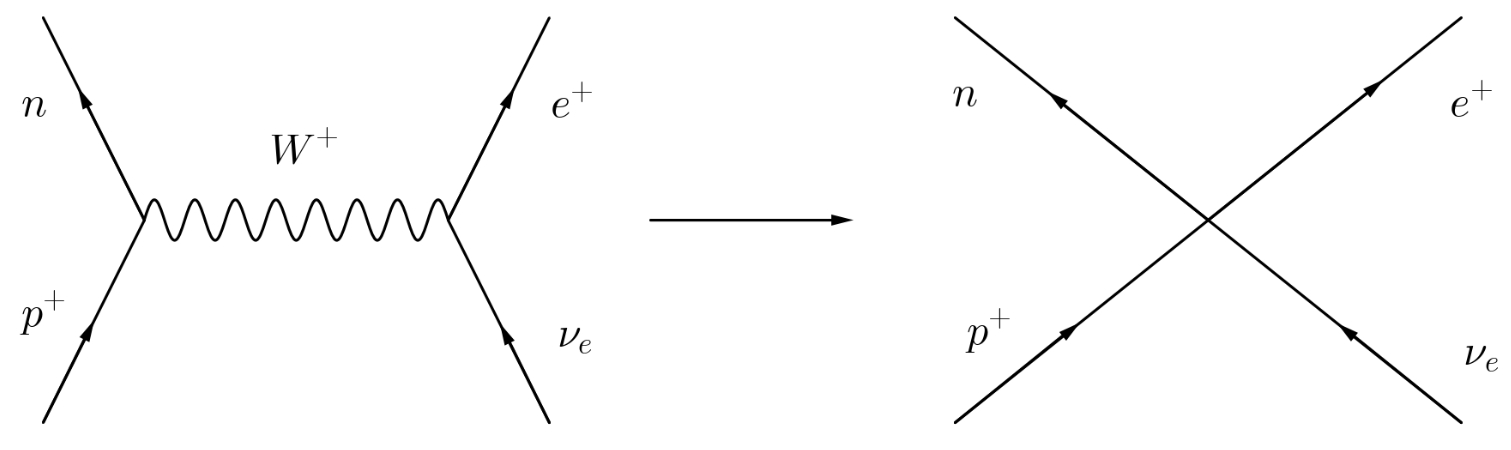
\includegraphics[width=0.8\textwidth]{Abbildungen/4fermi.jpg}
\caption{Feynman-Diagramme für GSW-Theorie (l.) und Fermi-Wechselwirkung (r.)}
\label{pic_4fermi}
\end{figure}
Zum hadronischen Strom kommt natürlich auch ein leptonischer Strom $l_\mu^c$, der im Aussehen seinem Pendant gleicht. Aus ihnen wird über eine Kopplungskonstante
ein hermitescher Hamiltonian konstruiert, der bereits in Abschnitt \ref{sec_fermigoldenrule} vorweg genommen wurde
\begin{equation}
 \mathcal{H} = \frac{G_F}{\sqrt{2}}\big(V^{c,\mu}\,l_\mu^{c\,\dagger} + l^{c,\mu}\,V_\mu^{c\,\dagger}\big),
\end{equation}
dessen Raumzeitstruktur als Vektor-Vektor-Kopplung (VV) bezeichnet wird. Die auftretenden Ströme verhalten sich unter Lorentz-Transformationen wie ein Raumzeit-Vektor.
Es zeigt sich, dass diese Art der Kopplung nicht die einzig lorentzinvariante ist. Aus bilinearen Kombinationen 4-komponentiger Spinoren ergeben sich 16 Freiheitsgrade,
die sich auf vektorielle (V), skalare (S), tensorielle(T), pseudoskalare (P) und axialvektorielle (A) Ströme verteilen. Aus den möglichen Kombinationen, Strom-Strom-Kopplungen zu erzeugen, gilt zu beachten, dass
der Hamiltonian (pseudo-)skalar sein muss, was die Kontrahierbarkeit beider Ströme erfordert. Eine dieser Kopplungen (VA) würde eine Paritätsverletzung erfordern,
da der Hamiltonian pseudoskalar ist und daher nicht mit dem Paritätsoperator vertauscht. Durch die Klärung des $\theta-\tau$-Rätsels und dem Experiment von Wu,
konnte die lang auf wissenschaftlichen Widerstand gestoßene Paritätsverletzung bestätigt werden.

\noindent
Der Helizitätsoperator für Fermionen $H$ als Skalarprodukt des Impulsoperators $\bar p$, der eine vektorielle Größe ist und dem Spinoperator $\vec \sigma$, 
der seinerseits ein Axialvektor ist, zeigt ebenfalls für Neutrinos die Paritätsverletzung. Positive und negative Helizität wären unter
Paritätsinvarianz gleich wahrscheinlich, jedoch ergibt sich aus dem Goldhaber-Experiment stets eine Helizität von $\langle H_\nu \rangle= -1$. Für relativistische
Invarianz muss ein entsprechender Operator gefunden werden. Bei masselosen, wie bei massiven Teilchen ergibt sich ein Projektionsoperator, der aus Spinoren 
die linkshändige Komponente extrahiert:
\begin{equation}
 \mathcal{P} = \frac12(1-\gamma_5),
\end{equation}
mit den Eigenschaften
\begin{equation}
 \mathcal{P}u_- = -u_- \qquad \text{und}\qquad \mathcal{P}u_+ = 0.
\end{equation}
Hieraus ergibt sich eine Erweiterung des bisher benutzten Leptonenstroms um linkshändige Neutrinos, die sich, wie in Abschnitt \ref{sec_fermigoldenrule}, schreiben lässt als
\begin{equation}
 l_\mu^c = \bar \psi_l \gamma_\mu (1-\gamma_5) \psi_\nu.
\end{equation}
Ebenfalls folgt eine Erweiterung des gesamten hadronischen Stroms $h_\mu^{c\,\dagger}$ in gleicher Form wie des leptonischen als
\begin{equation}
 h_\mu^{c\,\dagger} = \bar \psi_p \gamma_\mu(1-c_A\gamma_5)\psi_n,
\end{equation}
mit $c_A$ als ein von der inneren Struktur der nicht punktförmigen Hadronen abhängiger Faktor, der durch Renormierungseffekte der starken Wechselwirkung entsteht.
Der Faktor 1/2 fällt bei beiden schwachen Strömen nach Konvention weg. 
Beide Ströme enthalten neben dem ursprünglich allein gedachten Vektoranteil nun noch einen Axialvektoranteil, was sich in der Bezeichnung V-A-Struktur
niederschlägt.

\subsubsection{CKM-Matrix}
%\vspace{-0cm}
Durch die Paritätsverletzung zeigt sich, dass die geladenen, schwachen Ströme an linkshändige Teilchen und rechtshändige Antiteilchen koppeln \cite{DissForm}\cite{Sibold}. 
So liegt der Schluss nahe, Dubletts von Teilchen zu erzeugen, die in gleicher Stärke koppeln. Diese werden aus den zwei Leptonen aus je einer Generation 
($e$ und $\nu_e$, sowie $\mu$ und $\nu_\mu$) und dem Up- und Down-Quark gebildet. Das zu Beginn der CKM-Matrix-Entwicklung (Cabibbo, Kobayashi, Maskawa) 
bereits bekannte Strange-Quark
mit einem damals noch hypothetischen Charm-Quark zu einem Dublett zusammenzufassen, birgt Schwierigkeiten, da Mesonen mit einem $s$ bei einem leptonischen
Zerfall, beispielsweise $K^+(u\bar s) \rightarrow \mu^+ \nu_\mu$, dem damaligen Verständnis widersprechen. Mit der von Cabibbo entworfenen Idee, das $d$-
und das $s$-Quark als gedrehte Quarkzustände 
\begin{align}
 \begin{pmatrix}
  d'\\
  s'
 \end{pmatrix} = \begin{pmatrix}
		  \,\,\,d \cos \theta_c + s \sin \theta_c\\
		  -d \sin \theta_c + s\cos \theta_c
		  \end{pmatrix}
\end{align}
zu betrachten, ist die Erklärung dieses Flavourwechsels möglich und lässt sich in folgendem Strom ausdrücken
\begin{align}
 j^\mu &= (\bar u\, \bar c) \gamma^\mu (1-\gamma_5) U \begin{pmatrix}
                                                      d\\
                                                      s
                                                     \end{pmatrix},\\
 U &= \begin{pmatrix}
      \,\,\,\,\cos \theta_c\quad \sin \theta_c\\
      -\sin \theta_c\quad \cos \theta_c
     \end{pmatrix}.
\end{align}
Die Univeralität der Zerfallsamplitude $M$ aus \eqref{eq_fermiMG_F}, die bisher nur die Kopplungskontante $G_F$ besessen hat, hat nun noch den neuen Parameter
$\theta_c$, der Cabibbo-Winkel genannt wird. Dieser Winkel beschreibt den zusätzlichen Kopplungsfaktor der $W^\pm$-Bosonen an die schwachen 
Wechselwirkungseigenzustände $u, d', c, s'$ des $u$-,$d$-,$s$-, bzw. $c$-Quarks. Aus der Betrachtung von Zerfällen $u\rightarrow d$ und $c\rightarrow d$ lässt
sich $\theta_c \approx 13^\circ$ bestimmen. Die zweidimensionale Matrix $U$ ist zwar wegen Erhaltung der euklidischen Norm unitär, kann jedoch nicht die 
gefundene CP-Verletzung (Charge, Parity) erklären. Nach Kobayashi und Maskawa muss folglich eine dritte Fermionengeneration existieren,
die $U$ in eine 3$\times$3-Matrix erweitern würde, die zwar weiterhin unitär aber nun zusätzlich eine komplexe Phase $\e^{\text{i}\phi}$ enthalte. $V_{\text{CKM}}$ ist
ausdrückbar in der Standardparametrisierung, bei der die vier freien Parameter die eben genannte komplexe Phase und drei Eulerwinkel 
$\theta_{12} = \theta_c,\, \theta_{13}$ und $\theta_{23}$ sind. Die Wolfenstein-Parametrisierung beschreibt die CKM-Matrix ihrerseits mit den vier Parametern
$\lambda,\, A,\, \rho$ und $\eta$, welche die Verbindungen $\lambda = \sin\theta_{12},\, A\lambda^2 = \sin\theta_{23}$ und $A\lambda^3(\rho-\text{i}\eta) = \sin\theta_{13}\e^{-\text{i}\phi}$
haben.
\begin{align}
 V_{\text{CKM}} = \begin{pmatrix}
            V_{ud}\,V_{us}\,V_{ub}\\
            V_{cd}\,V_{cs}\,V_{cb}\\
            V_{td}\,V_{ts}\,V_{tb}\\
           \end{pmatrix} = \begin{pmatrix}
			    1-\frac12\lambda^2 & \lambda & \lambda^3A(\rho-\text{i}\eta)\\
			    -\lambda & 1-\frac12 \lambda^2 &\lambda^2A\\
			    \lambda^3A(1-\rho-\text{i}\eta) &-\lambda^2A & 1
			    \end{pmatrix}
\end{align}
Sollte die CP-Verletzung einzig aus der komplexen Phase kommen, lässt sich zeigen, dass CP-verletzende Amplituden proportional zur Fläche des sogenannten
Unitaritätsdreiecks sind. Es handelt sich hierbei um ein Dreieck in der komplexen Ebene mit $\rho$ und $\eta$ als Achsen. Die Seiten werden durch Komponenten
von $V_{\text{CKM}}$ repräsentiert.

\section{Parametrisieren von Formfaktoren}
\label{sec_paramForm}
Der wie in Abschnitt \ref{sec_fermiWW} dargestellte hadronischen Strom $h_\mu^{c\dagger}$ lässt sich aufgrund von starken Wechselwirkungen zwischen den 
Hadronkonstituenten nicht so einfach schreiben, sondern wird wie in Abschnitt \ref{sec_fermigoldenrule} bereits vorweggenommen, durch einheitenlose Formfaktoren 
ausgedrückt\cite{KimPham}. Der Sachverhalt wird am für den betrachteten Zerfall relevanten Feynmangraphen in Abbildung \ref{pic_Dfeyn} dargestellt.
\begin{figure}[H]
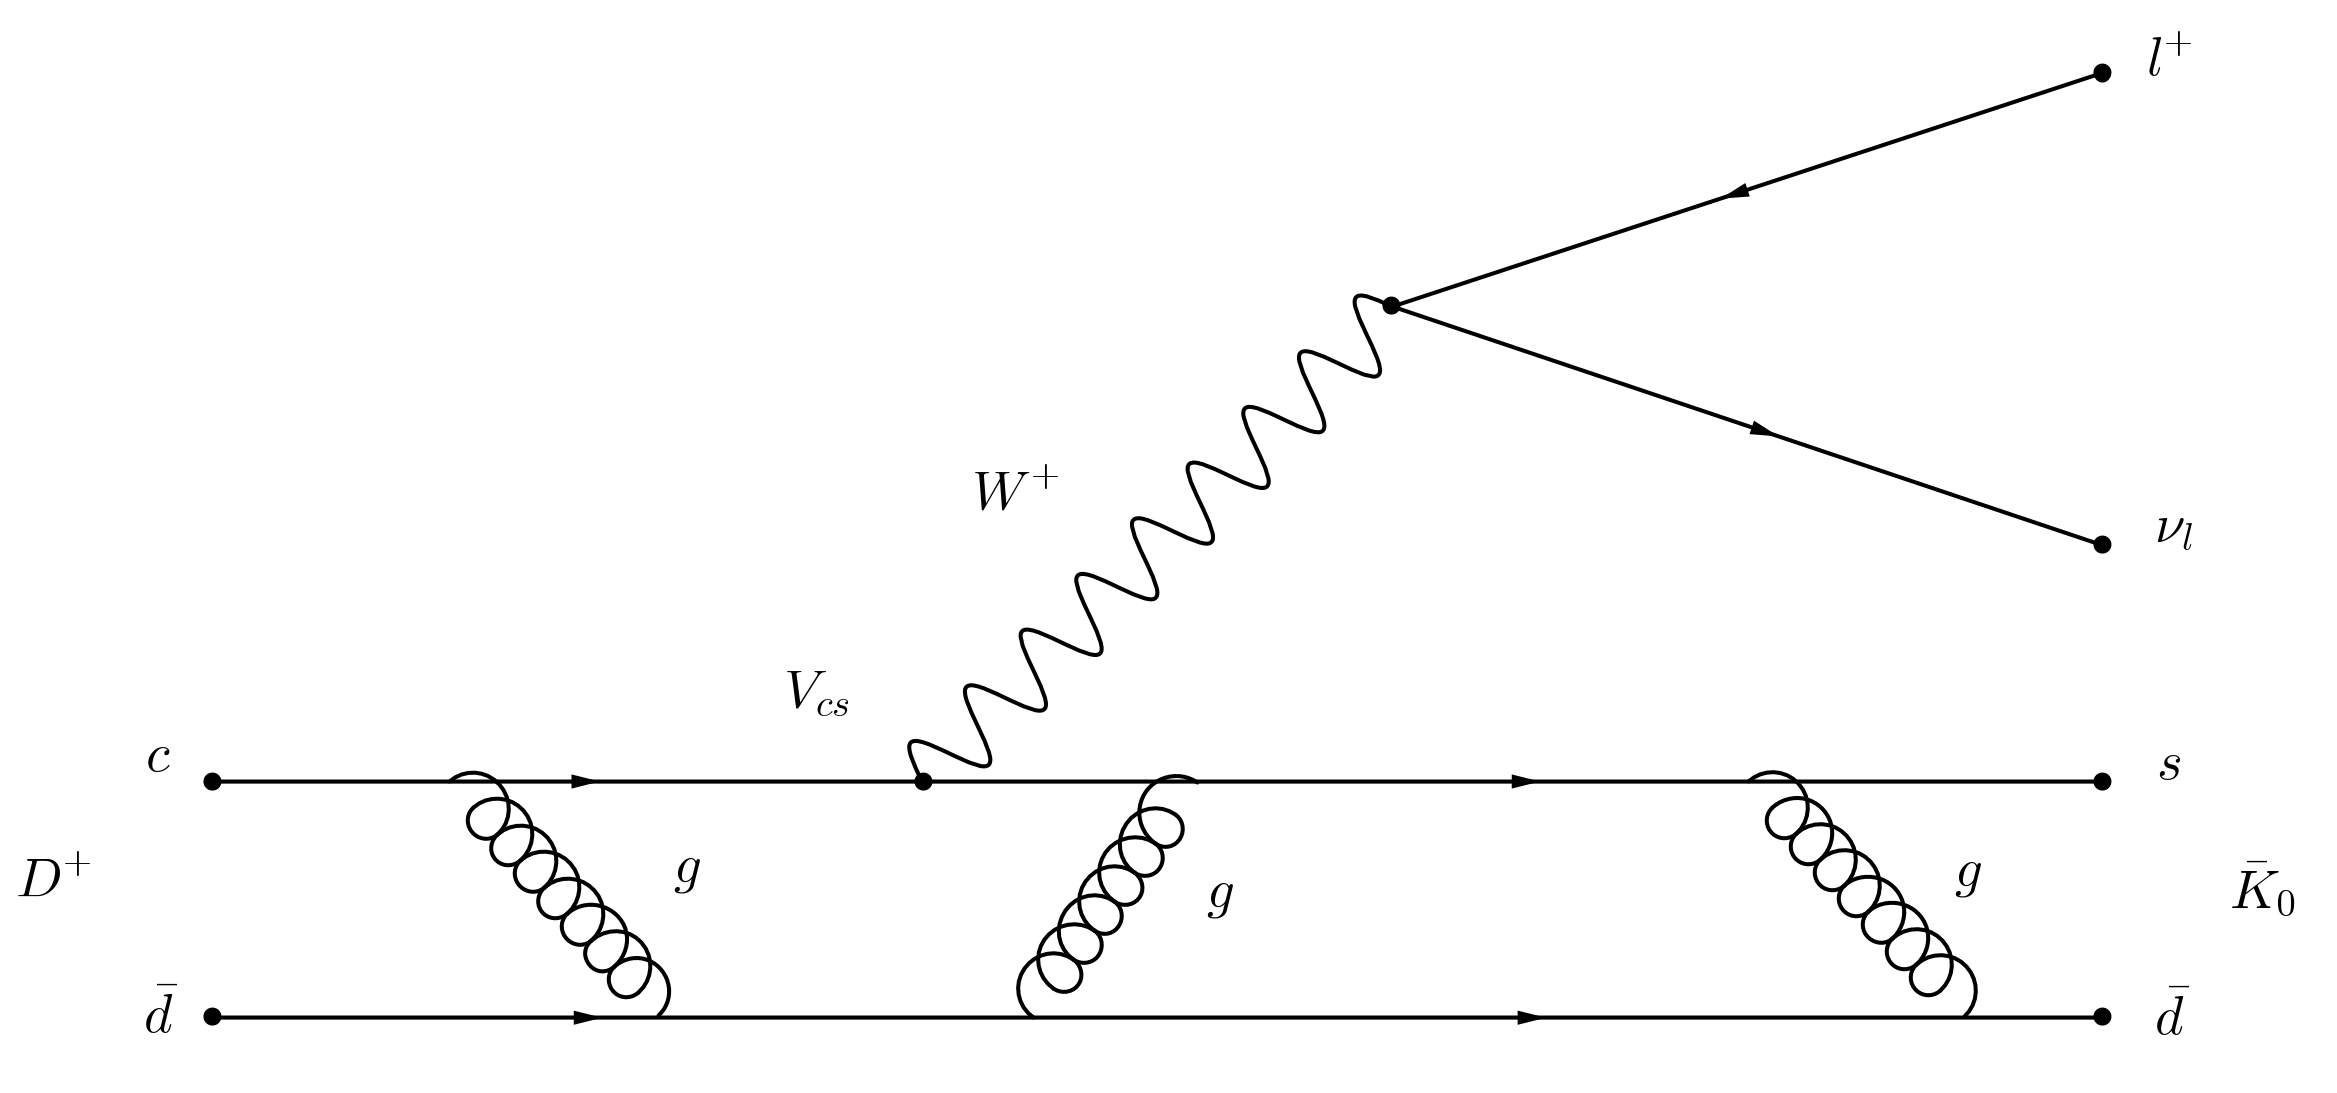
\includegraphics[width=0.8\textwidth]{Abbildungen/DFeyn.png}
\caption{Feynmangraph zum $D\rightarrow \bar K l^+ \nu_l$ Zerfall.}
\label{pic_Dfeyn}
\end{figure}
\noindent
So ist die Betrachtung einer Vier-Fermionen-Wechselwirkung unzureichend, da die Austauschbosonen der QCD, die Gluonen $g$, einen störungstheoretisch nicht
ermittelbaren Einfluss auf den schwachen Zerfall haben.
In einem Zweikörper-Zerfall $E\rightarrow PQ$ sind zwei Freiheitsgrade möglich, die den Prozess charakterisieren. Dies sind die Viererimpulse des Eduktteilchens
$p_E$ und des Produktteilchens $p_P$, da der Viererimpuls des verliebenen Produktteilchens $q$ von den vorigen determiniert wird. Da der vektorielle 
Anteil des schwachen Stroms $V^\mu$ aus \eqref{eq_fermiMG_F} nicht erhalten ist (WAS HEISST DAS GENAU?), gibt es hierbei zwei Formfaktoren $f_\pm$, die der allgemeinsten Form
dessen Beschreibung dienen
\begin{align}
 \big\langle K(p_K)\,\big|V^\mu\big|\, D(p_D)\big\rangle = f_+(q^2)(p_D+p_K)^\mu + f_-(q^2)(p_D-p_K)^\mu.
\end{align}
Es gibt viele Ansätze, diese Formfaktoren zu bestimmen. Neben dem theoretischen Weg über die Gitterquantenchromodynamik, existieren einige Parametrisierungen,
die anhand experimenteller Daten einen Zugang ermöglichen. Die Pol-Parametrisierungen weisen ein schlechtes Konvergenzverhalten nahe der semileptonischen Bereiche
des Impulsübertrags $q^2$ auf, was Zweifel an einer korrekten Berechnung des Formfaktors übrig lässt \cite{PhysRev_Data}. Eine Darstellung, die ein solches Problem nicht hat,
ist eine sogenannte $z$-Reihenentwicklung \cite{formfactor_PhysRev}
\begin{align}
 f(q^2) = \frac{1}{1-\frac{q^2}{m^{*2}_D}} \sum\limits_{i=0}^\infty a_i\,z^i(t_0,\, q^2).
 \label{eq_formparam}
\end{align}
Die Koeffizienten $a_i$ sind
aus einem Fit zu bestimmende Größen. die Konvergenz der Reihe wird dadurch gesichert, dass $|z|<1$ im physikalischen Bereich. Sie wird dargestellt durch
\begin{align}
 z(t_0,\, q^2)= \frac{\sqrt{t_+-q^2}-\sqrt{t_+-t_0}}{\sqrt{t_+-q^2}+\sqrt{t_+-t_0}},
 \label{eq_zexpansion}
\end{align}
worin $t_\pm$ bestimmt sind durch $t_\pm = (m_D \pm m_K)$ und $t_0$ als ein konstantes Optimum gewählt wird, was klassischerweise zu 
$t_0 = t_+(1-(1-t_-/t_+)^{1/2})$ bestimmt wird, da es den Maximalwert von $z(t_0,\, q^2)$ minimiert.

\noindent
Bei Übergängen mit nicht verschwindendem Axialvektorstrom $A^\mu$, wie zum Beispiel von einem pseudoskalaren zu einem vektoriellen Teilchen, treten 
weitere Formfaktoren auf. Die Ausdrücke für diesen Strom und die Abhängigkeiten der Formfaktoren $A_i(q^2)$ sind teilweise sehr komplex, sodass wegen
der hier nicht bestehenden Relevanz nicht näher darauf eingegangen wird.

\chapter{Ergebnisse}
Die zahlreichen, möglichen Formfaktoren des betrachteten Zerfalls werden im folgenden diskutiert, nachdem der physikalisch mögliche Bereich des Impulsübertrags
berechnet worden ist. So werden die Axialvektorformfaktoren unter Paritätsbetrachtungen und $f_-$ aufgrund von vernachlässigbarer Leptonenmassen verschwinden.
Schließlich wird der einzig verbliebene Formfaktor $f_+$ unter Minimierung einer $\chi^2$-Funktion bestimmt.
\section{Kinematische Größen}
%\vspace{-1.7cm}
Die Formfaktoren werden allgemein in Abhängigkeit des Impulsübertrags $q^2$ angegeben. Da dieser nicht beliebige Werte annehmen kann, ist es sinnvoll, den 
möglichen Wertebereich zu ermitteln.  In Abbildung \ref{pic_DZerfall} sind die beiden Randbereiche dargestellt. Im linken Teil des Bildes befindet sich das 
entstehende Kaon wieder in Ruhe und im rechten Teil nimmt es die gleiche Menge an Impuls auf, wie das Leptonenpaar.
\begin{figure}[H]
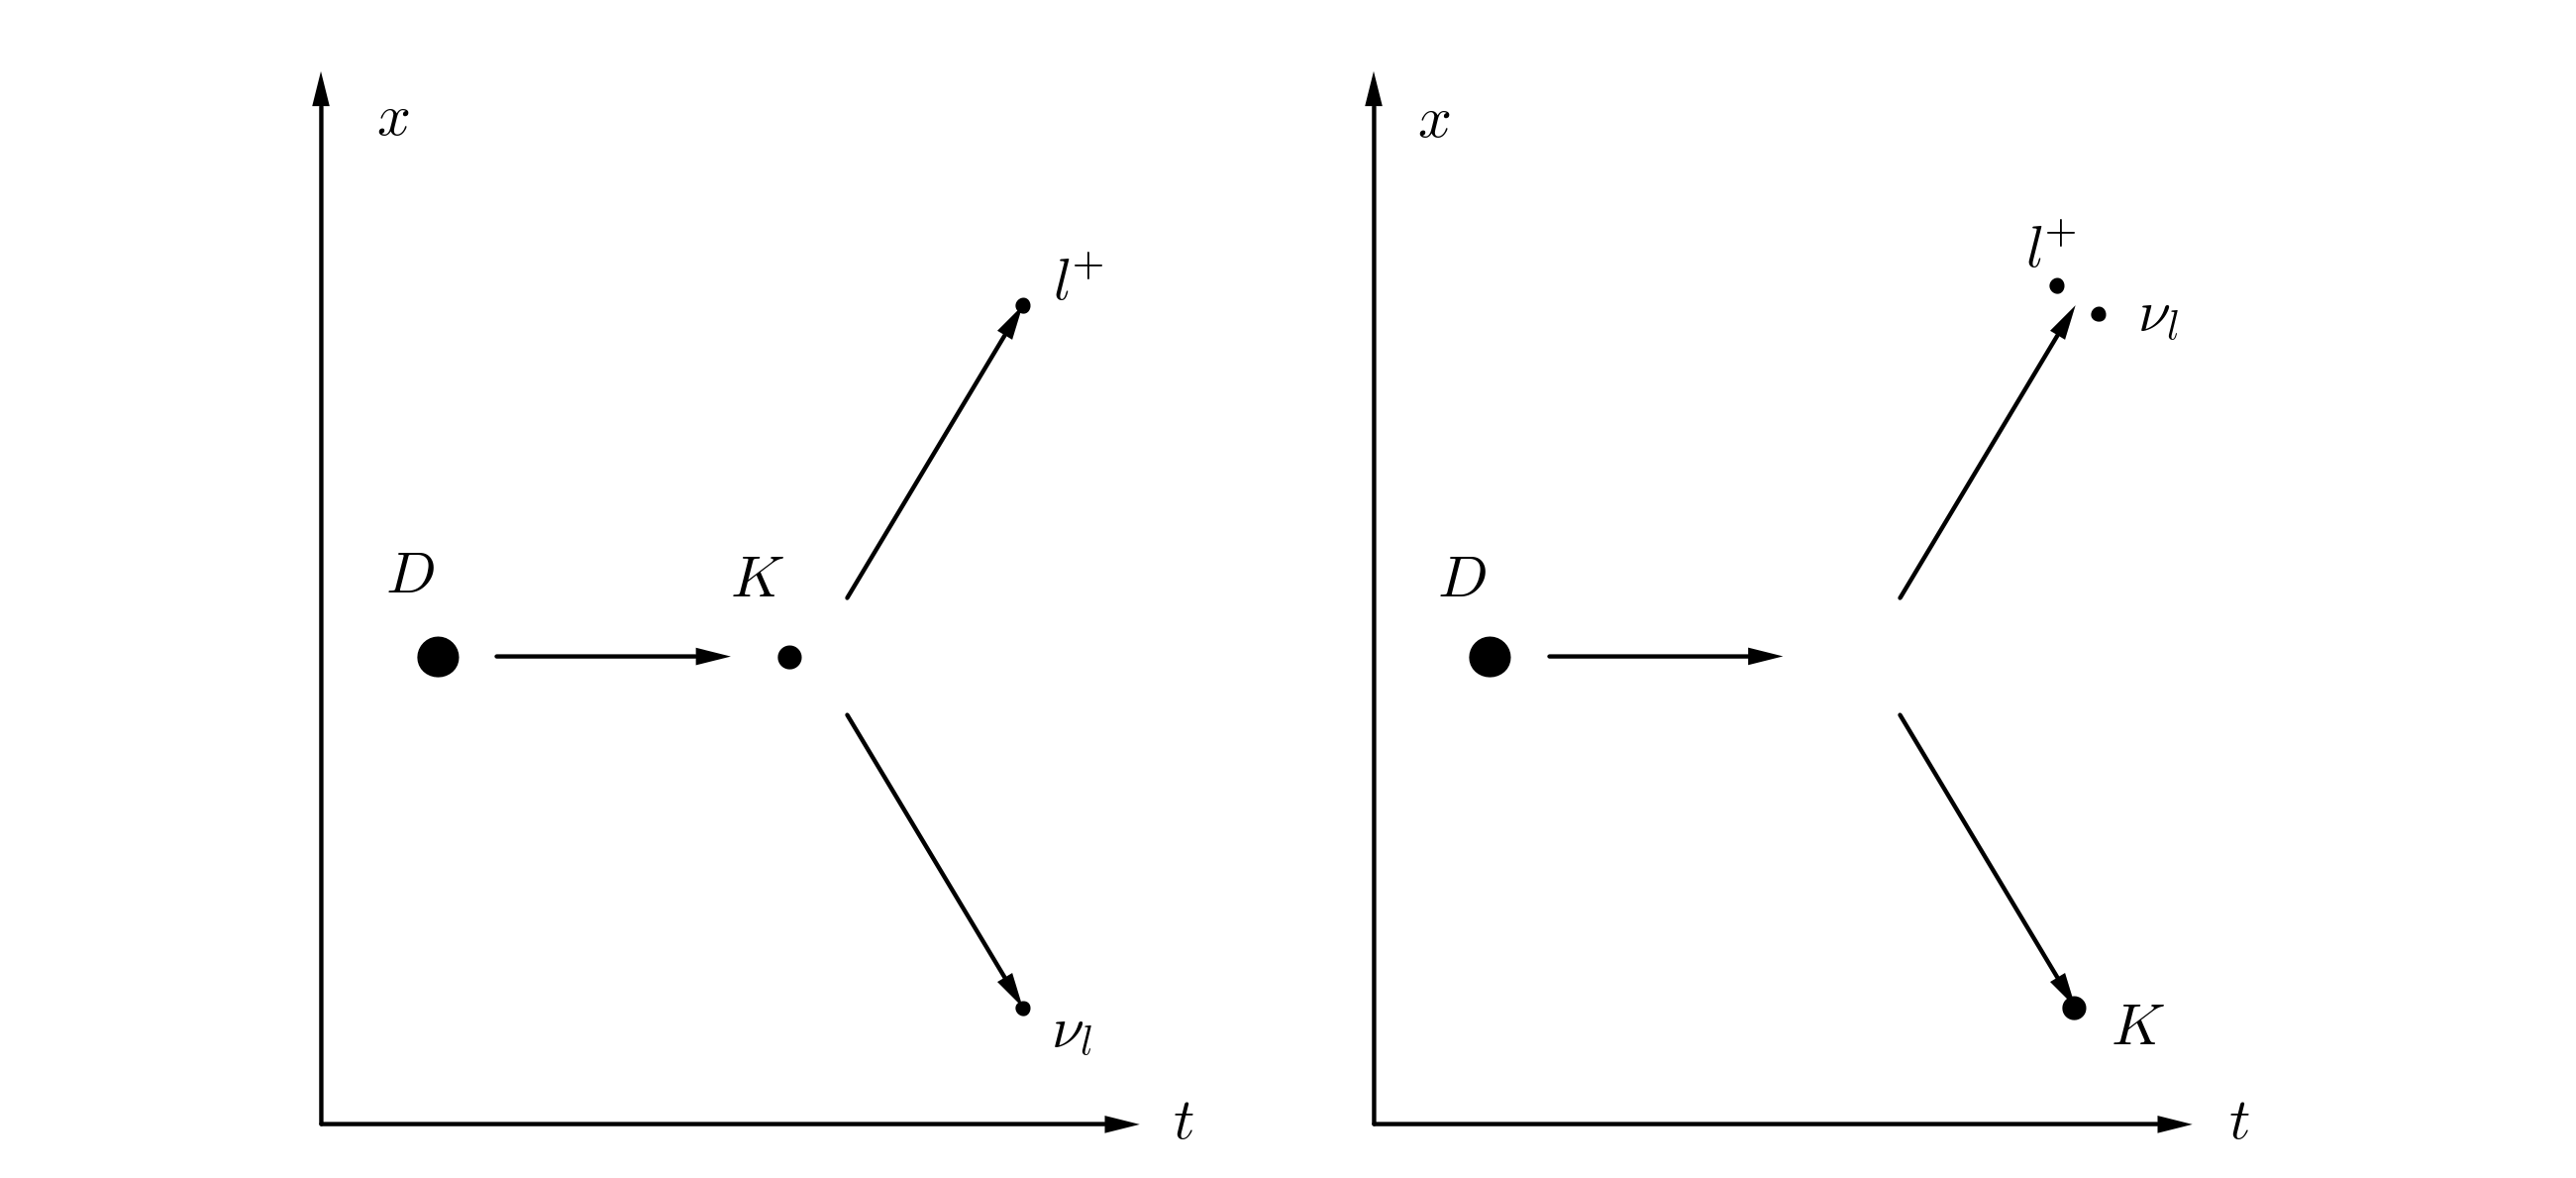
\includegraphics[width=1\textwidth]{Abbildungen/DZerfall.png}
\caption{Zwei Zerfallsmöglichkeiten des $D^+$-Mesons  mit extremen $q^2$-Werten.}
\label{pic_DZerfall}
\end{figure}
\noindent
Zur Berechnung wird entsprechend den Regeln der Vierer-Impuls-Algebra die Vierer-Impuls-Erhaltung im Ruhesystem des D-Mesons betrachtet
\begin{align}
 p_D^\mu &= p_K^\mu + p_l^\mu + p_\nu^\mu \nonumber\\
 p_D^\mu - p_K^\mu &= q^\mu = p_l^\mu + p_\nu^\mu \nonumber\\
 \left(p_D^\mu-p_K^\mu\right)^2 &= q^2 =  (p_l^\mu + p_\nu^\mu )^2\nonumber\\
 m_D^2 + m_K^2 - 2m_DE_K &= q^2 = m_l^2 + m_\nu^2 + E_lE_\nu - |\vec p_l||\vec p_\nu|\cos(\xi).
\end{align}
An diesem Ausdruck lässt sich der in Abschnitt \ref{sec_fermigoldenrule} verwandte Zusammenhang $\dx E = \dx q^2/2m_D$ erkennen.
Sollte das Kaon sich nach dem Zerfall in Ruhe befinden, so ist $E_K = m_K$, woraufhin $q^2 = (m_D-m_K)^2$ wäre. Für vernachlässigbare Leptonmassen 
($m_l=m_\nu=0$), gilt $E=|\vec p|$ und $q^2$ verschwindet , falls die Impulsrichtungen der Leptonen in die gleiche Richtung zeigen, also der Zwischenwinkel
$\xi = 0$. Es resultiert ein Wertebereich von
\begin{equation}
 0 \leq q^2 \leq (m_D - m_K)^2.
\end{equation}

\section{Die Axialvektorformfaktoren und $f_-$}
Wie an manchen Stellen bereits erwähnt und vorausgesetzt, verschwinden die Formfaktoren des Axialvektorstroms. Formfaktoren beschreiben starke 
Wechselwirkungen zwischen dem zerfallenden Quark (hier $c$) und dem Spectatorquark (hier $\bar d$, $\bar u$), was heißt, dass die Parametrisierung des 
Vektor- und Axialvektorstroms dasselbe Paritätstransformationsverhalten haben müssen. Die Ströme besitzen ein Paritätsverhalten von
\begin{align}
 \mathcal{P} \, \big\langle\bar K^0\,\big|V^\mu|\,D^+\big\rangle &= (-1)\cdot(-1)\cdot(-1) = -1 \nonumber \\
 \mathcal{P} \, \big\langle\bar K^0\,\big|A^\mu|\,D^+\big\rangle &= (-1)\cdot(+1)\cdot(-1) = +1. \nonumber
\end{align}
Aus den beiden einzigen Freiheitsgraden des Zerfalls, den Impulsen $p$ und $p'$, und dem Levi-Civita-Symbol $\epsilon^{\mu\nu\alpha\beta}$ lassen sich alle möglichen
Darstellungen von Strömen mit unbestimmten Vorfaktoren schreiben als
\begin{align}
 \underbrace{p^\mu}_{V} + \underbrace{p'^\mu}_{V}+ \underbrace{p^\mu p'_\mu }_{S} + \underbrace{\epsilon^{\mu\nu\alpha\beta}p_\alpha p'_\beta}_{T},
\end{align}
wobei die Größen unter den Klammern das entsprechende Transformationsverhalten angeben. Daraus ergibt sich, dass die einzigen vektoriellen Beiträge wie 
Vektoren $V$ und keiner wie Axialvektoren $A$ transformieren. Damit ein solcher Beitrag existieren könne, müsse er aufgrund seiner Eigenschaft $J^P = 1^+$
eine Struktur haben, wie $A^\mu = \epsilon^{\mu\alpha\beta\gamma}p_\alpha\,p'_\beta\,p''_\gamma$ mit einem weiteren Freiheitsgrad $p''$. Da dieser zur 
Konstruktion jedoch nicht vorhanden ist, verschwindet der Axialvektoranteil.

\noindent
Um nachzuvollziehen, was mit $f_-$ geschieht, wird das Matrixelement aus \eqref{eq_fermiMG_F} ohne $f_+$ betrachtet. Der Impulsübertrag $q$ ist nicht
nur die Differenz der mesonischen Viererimpulse, sondern auch die Summe der leptonischen
\begin{align}
 M_- &= \frac{G_F V}{\sqrt{2}} f_-(q^2)(p_D-p_K)^\mu u_\nu \gamma_\mu(1-\gamma_5)v_l\nonumber\\
 &= \frac{G_F V}{\sqrt{2}} f_-(q^2)(k_\nu+k_l)^\mu u_\nu \gamma_\mu(1-\gamma_5)v_l.\nonumber
\end{align}
Unter Einbezug des leptonischen Stroms ersetzt die Dirac-Gleichung \eqref{eq_dirac} die $k_i$ durch die zugehörigen Massen
\begin{align}
 &=\frac{G_F V}{\sqrt{2}} f_-(q^2)u_\nu (\slashed{k}_\nu + \slashed{k}_l) (1-\gamma_5)v_l\nonumber\\
 &=\frac{G_F V}{\sqrt{2}} f_-(q^2)u_\nu (m_\nu + m_l) (1-\gamma_5)v_l,\nonumber 
 \end{align}
die im Verhältnis zur $D$-Mesonmasse für $l=\mu$ oder $l=e$ vernachlässigbar sind, woraufhin $M_-$ verschwindet.

\section{Fit des Formfaktors $f_+$}
In Abschnitt \ref{sec_fermigoldenrule} ist ein kompakter Ausdruck für den Zusammenhang der differentiellen Zerfallsrate und dem 
Formfaktor $f_+$ hergeleitet worden. Da der Formfaktor nicht leicht analytisch berechenbar ist, wird er entsprechend der Parametrisierung \eqref{eq_formparam}
nach der Methode der kleinsten Quadrate an den experimentell erhobenen Daten für die partiellen Zerfallsraten gefittet. Im Rahmen der Messmethoden, ist es
nicht möglich, eine genaue Zuordnung eines gemessenen Zerfalls zum entsprechenden Impulsübertrag zu erreichen, weshalb die Zerfallsraten für diskrete Bereiche
angegeben werden. 

\subsection{Methode der kleinsten Quadrate}
Die Aufgabe des Fits liegt darin, die Funktion zu finden, die am geringsten von den Messwerten abweicht. Dies geschieht über die Minimierung einer
Funktion $\chi^2$, die durch die Summe über die Anzahl diskreter Intervalle $m$ vom Produkt aus Differenzen experimenteller Daten $\Delta \Gamma$ und 
zugehörigen, theoretischen Vorhersagen $g$, verknüpft über die Inverse einer Kovarianzmatrix $C$ gegeben ist.
\begin{align}
 \chi^2 = \sum\limits_{i,j=1}^m (\Delta \Gamma_i - g_i(f_+))C^{-1}_{ij}(\Delta \Gamma_j - g_j(f_+)).
\end{align}
Von der nie ganz abschirmbaren Hintergrundstörung, Strahlungen der Endteilchen (FSR) oder Monte Carlo Simulationen (MC), die zur Rekonstruktion von 
Teilchenpfaden in Detektoren genutzt werden, entstehen Fehlerquellen $\sigma$ für die individuellen Zerfallsraten, die ebenso, wie die Messwerte 
\cite{PhysRev_Data} $\Delta \Gamma$ in Tabelle \ref{tab_GammaSigma} mit den zugehörigen $q^2$-Intervallen angegeben sind. Die 
Zuordnung der Zerfallsraten zu den $q^2_i$ erfolgt leider ebenfalls nicht fehlerfrei. Die dadurch entstehenden Korrelationen zwischen diesen Intervallen 
sind teils statistischer und teils systematischer Natur, deren Matrixdarstellungen in den Tabellen \ref{tab_corStatDplus} bis \ref{tab_corSysD0} zu finden 
sind. Die zu invertierende Kovarianzmatrix setzt sich additiv aus den Kovarianzmatrizen mit den statistischen bzw. den systematischen Beiträgen zusammen
\begin{align}
 C = C^{\text{stat}} + C^{\text{sys}}.
\end{align}
Ihre jeweiligen Einträge ergeben sich aus den kennzeichnenden Korrelationsmatrixeinträgen und den entsprechenden Kovarianzen
\begin{align}
 C^{\alpha}_{ij} = \sigma^{\alpha}_i \sigma^{\alpha}_j \cdot \rho^{\alpha}_{ij}, \hspace{2cm}\alpha = \text{stat, sys}.
\end{align}
Die Funktion des hier verwandten, theoretischen Modells stellt das Integral der differentiellen Zerfallsbreite über $q^2$ dar und berechnet sich aus 
\eqref{eq_fermidGammafinal} zu
\begin{align}
 g_i(f_+) = \Gamma_{\text{theo},i} = \frac{G_F^2 |V_{cs}|^2}{24\pi^3}\int|p_K(q_i^2)|^3 \cdot |f_+(q^2_i)|^2\dx q_i^2,
\end{align}
das sich zwar nicht analytisch, jedoch aufgrund der guten Konvergenzeigenschaften der beitragenden Terme auf numerischem Weg lösen lässt. 

\subsection{Resultate für die Koeffizienten und den Startwert}
\renewcommand{\arraystretch}{1.2}
\begin{table}[H]
  \begin{tabular}{l|ccc|crc}
  \toprule
    \multirow{2}{*}{$q^2$ in GeV$^2$}& \multicolumn{3}{c|}{$D^+ \rightarrow \bar K_0 l^+ \nu$} & \multicolumn{3}{c}{$D^0 \rightarrow  K^- l^+ \nu$}\\
    \cline{2-7}
    & $\Delta \Gamma$ in ns$^{-1}$ & $\sigma^\text{sys}$ & $\sigma^\text{stat}$ & $\Delta \Gamma$ in ns$^{-1}$ & $\sigma^\text{sys}$ & $\sigma^\text{stat}$\\
   \midrule
  {[}0,0 - 0,4) & 	17,82(36)&	2,03&	1,26&	17,79(47)&	2,03&	2,52 \\
  {[}0,2 - 0,4)& 	15,83(35)&	2,19&	1,10&	15,62(45)&	2,19&	2,42\\
  {[}0,4 - 0,6) &	13,91(32)&	2,31&	1,12&	14,02(43)&	2,31&	2,36\\
  {[}0,6 - 0,8) & 	11,69(29)&	2,47&	1,15&	12,28(40)&	3,23&	2,33\\
  {[}0,8 - 1,0)  &	9,36(26)&	2,73&	1,20&	8,92(34)&	3,82&	2,47\\
  {[}1,0 - 1,2)  &	7,08(22)&	3,14&	1,36&	8,17(32)&	3,98&	2,23\\
  {[}1,2 - 1,4)  &	5,34(19)&	3,63&	1,35&	4,96(25)&	5,04&	2,08\\
  {[}1,4 - 1,6)  &	3,09(15)&	4,90&	1,63&	2,67(18)&	6,88&	2,16\\
  {[}1,6 - $\infty$)&	1,28(11)&	8,43&	2,55&	1,19(13)&	10,63&	3,03\\
  \bottomrule\bottomrule
  \end{tabular}
\caption{Gemessene partielle Zerfallsraten bei entsprechenden Impulsüberträgen und zugehörigen systematischen und statistischen Kovarianzen für beide Zerfallskanäle}
\label{tab_GammaSigma}
\end{table}



\chapter{Zusammenfassung und Ausblick}

Hier sollen die Ergebnisse zusammengefasst und weiterf\"uhrende Untersuchungen diskutiert werden. 

mit anderen zerfällen ist Vcs extrahierbar
% >>> Anhang <<<

\begin{appendix}
%\input{Kapitel/Anhang}
\end{appendix}
\newpage
% >>> Literaturverzeichnis <<<


\renewcommand{\bibname}{Literaturverzeichnis}
\addcontentsline{toc}{chapter}{\bibname}
%\bibliographystyle{unsrt} 
%\bibliography{BachelorArbeit}
\begin{thebibliography}{xxx}
 \bibitem[1]{RelKin}Nedden zur, M.: \textit{Detektoren der Elementarteilchenphysik}[pdf], 2006\\ \href{http://www-hera-b.desy.de/people/nedden/lectures/05_06/dettph/dettph_cont.pdf}{http://www-hera-b.desy.de/people/nedden/lectures/05\_06/dettph/dettph\_cont.pdf}
 \bibitem[2]{TeilFortgeschr}Schleper, P.: \textit{Teilchenphysik für Fortgeschrittene}[pdf], 2011\\ \href{http://www.desy.de/~schleper/lehre/}{http://www.desy.de/\midtilde schleper/lehre/}
 \bibitem[3]{RelQuantMech}Bjorken, J.D., Drell, S.D.: \textit{Relativstic Quantum Mechanics}, 1964, 1st edition \\ISBN-13 978-0072320022 
 \bibitem[4]{Griffiths}Griffiths, D.: \textit{Introduction to Elementary Particles}, 2008, 1st edition \\ISBN-13 978-3527406012
 \bibitem[5]{PDG} Beringer, J. et al.: \textit{Particle Data Group}, Phys. Rev. D86, 010001, 2012
 \bibitem[6]{Klapdor}Grotz, K., Klapdor H.V.: \textit{Die schwache Wechselwirkung in Kern-, Teilchen- und Astrophysik}, 1989, 1st edition, ISBN-13 978-3519030355
 \bibitem[7]{DissForm}Offen, N.: \textit{B-Zerfallsformfaktoren aus QCD-Summenregeln}, 2008\\ \href{http://d-nb.info/987811061}{http://d-nb.info/987811061}
 \bibitem[8]{Sibold}Sibold, K.: \textit{Theorie der Elementarteilchen}, 2001, 1st edition, \\ISBN-13: 978-3519032526
 \bibitem[9]{KimPham}Ho-Kim, Q., Pham, X.: \textit{Elementary Particles and Their Interactions}, 1998, \\ ISBN-13: 978-3540636670
 \bibitem[10]{PhysRev_Data}Besson, D., et al. (CLEO Collaboration), 2009, Phys. Rev. D 80, 032005 
 \bibitem[11]{formfactor_PhysRev}Bourrely, C., Caprini, I., Lellouch, L., 2009, Phys. Rev. D 79, 013008
\end{thebibliography}



\newpage
\thispagestyle{empty}
\ \\

% >>> Erklaerung <<<

\thispagestyle{empty}
\begin{center}
\section*{Eidesstattliche Versicherung}
\end{center}
\vspace*{1cm}
\noindent
Ich versichere hiermit an Eides statt, dass ich die vorliegende Bachelorarbeit mit dem Titel ''{\thetitle}'' selbst\"andig und ohne unzul\"assige fremde Hilfe erbracht habe. Ich habe keine anderen als die angegebenen
Quellen und Hilfsmittel benutzt sowie w\"ortliche und sinngem\"a\ss e Zitate kenntlich gemacht.
Die Arbeit hat in gleicher oder \"ahnlicher Form noch keiner Pr\"ufungsbeh\"orde vorgelegen.
\vspace*{1cm}
\ \\
\ \\
\line(1,0){150} \hfill \line(1,0){150}\\
Ort, Datum \hfill Unterschrift \hspace*{3cm}
\vspace*{1.5cm}

\subsection*{Belehrung}
Wer vors\"atzlich gegen eine die T\"auschung \"uber Pr\"ufungsleistungen betreffende Regelung einer Hochschulpr\"ufungsordnung
verst\"o\ss t handelt ordnungswidrig. Die Ordnungswidrigkeit kann mit einer Geldbu\ss e von bis zu \unit[50.000,00]{\euro} geahndet werden. Zust\"andige Verwaltungsbeh\"orde f\"ur die Verfolgung und Ahndung von Ordnungswidrigkeiten ist
der Kanzler/die Kanzlerin der Technischen Universit\"at Dortmund. Im Falle eines mehrfachen oder sonstigen schwerwiegenden T\"auschungsversuches kann der Pr\"ufling zudem exmatrikuliert werden (\S\ 63 Abs. 5 Hochschulgesetz - HG - ).\\
\ \\
Die Abgabe einer falschen Versicherung an Eides statt wird mit Freiheitsstrafe bis zu 3 Jahren oder mit Geldstrafe bestraft.\\
\ \\
Die Technische Universit\"at Dortmund wird ggf. elektronische Vergleichswerkzeuge (wie z.B. die Software ''turnitin'') zur \"Uberpr\"ufung von Ordnungswidrigkeiten in Pr\"ufungsverfahren nutzen.\\
\ \\
Die oben stehende Belehrung habe ich zur Kenntnis genommen.
\vspace*{1cm}
\ \\
\ \\
\line(1,0){150} \hfill \line(1,0){150}\\
Ort, Datum \hfill Unterschrift \hspace*{3cm}
\vspace*{\fill}
\end{spacing}

\end{document}